\documentclass[11pt,xcolor={dvipsnames},aspectratio=159,hyperref={pdftex,pdfpagemode=UseNone,hidelinks,pdfdisplaydoctitle=true},usepdftitle=false]{beamer}
\usepackage{presentation}[aspectratio=169]
\usepackage{math}
\usepackage{mathtools}
\usepackage{mleftright}
% Enter title of presentation PDF:
\hypersetup{pdftitle={Government Spending Multiplier: Theory II and Empirical Results}}
% Enter link to PDF file with figures:

\begin{document}
% Enter presentation title:
\title{Government Purchases Multiplier: Theory and Empirical Results}
\subtitle{Fiscal and Monetary Policy 2024}
% Enter presentation information:

% Enter presentation authors:
\author{Piotr Żoch}%
% Enter presentation location and date (optional; comment line if not needed):
\frame{\titlepage}

% Fill out content of presentation:

\begin{frame}
    \heading{Beyond the NGM}
\end{frame}

\begin{frame}{Real rates}
    \begin{itemize}
    \item Consider the Euler equation 
\begin{align*}
    \frac{u'\of{c_t}}{u'\of{c_{t+1}}} = \beta\bp{1 + r_{t+1}}.
\end{align*}
\item We said that consumption growth is determined by the real interest rate.
\item In NGM the real rate was tied to the marginal product of capital: $$r_t = F_1\of{k_t,n_t} - \delta.$$ 
\end{itemize}
\end{frame}

\begin{frame}{Real rates}
    \begin{itemize}
    \item Suppose that the government can \al{somehow} control the real rate and keeps it constant at the steady state level $r=\beta^{-1}-1$.
    \item Then the Euler equation becomes \begin{align*}
        \frac{u'\of{c_t}}{u'\of{c_{t+1}}} = 1,
    \end{align*}
    which implies that consumption is constant.
    \item In this case the multiplier will depend only on the response of $i_t$ to $g_t$. 
    \item If investment is constant, then the multiplier will be equal to one.
\end{itemize}
\end{frame}      

\begin{frame}{Real rates}
    \begin{itemize}
    \item Consider a special case with no capital in this economy (or: fixed capital). 
    \item The multiplier depends \al{only} on the behavior of the real rate.
    \item Nothing else matters. 
    \item This is what happens in a large class of representative agent New Keynesian models (RANK) (which we will discuss later). 
    \item Monetary policy response to government purchases is crucial, because it affects the real rate. See Woodford (2011). 
    \end{itemize}
\end{frame}

\begin{frame}{Real rates}
    \begin{itemize}
    \item Note: this holds \al{regardless} of how the government finances its spending.
    \item It is not the balanced budget multiplier. 
    \item This result hinges on the presence of the Euler equation for aggregate consumption and $$y_t = c_t + g_t.$$
    \end{itemize}
\end{frame}      

\begin{frame}{Taking stock}
    \begin{itemize}
    \item We saw that multipliers in a NGM seem to be at odds with the usual Keynesian cross analysis.
    \item We also noticed the key role of real rates in determining the multiplier.
    \item Does it mean that the Keynesian cross analysis was invalid and we cannot have a simple framework to analyze fiscal policy?
    \item Not really, but we need to be more careful and take into account the intertemporal nature of consumption-savings decisions. 
    \end{itemize}
\end{frame}      

\begin{frame}
    \heading{Auclert, Rognlie, and Straub (2024): \\The Intertemporal Keynesian Cross (IKC)} 
        \end{frame}

  

\begin{frame}{IKC}
    \begin{itemize}
        \item Key insight: \al{intertemporal marginal propesnsities to consume} (iMPCs) are \alb{sufficient statistics} for the effect of fiscal policy.
        \item Fiscal multipliers depend on the interaction of public deficits and iMPCs.
        \item If we want to know the effect of fiscal policy, we should measure iMPCs in the data - or at least use models that generate iMPCs roughly consistent with the data.
    \end{itemize}
    
\end{frame}

\begin{frame}{Household}
    \begin{itemize}
     \item Household $i$ solves:
     \begin{align*}
        \max_{\bc{c_{i,t},b_{i,t}}} & \E_0 \sum_{t=0}^\infty \beta^t \bp{u\of{c_{i,t}}- \nu\of{h_{i,t}}} \\
        & b_{i,t} + c_{i,t} = \bp{1+r^B_{t}} b_{i,t-1} + z_{i,t} \bp{1-\tau_t}\frac{W_t}{P_t} h_{i,t} \\
        & b_{i,t} \geq \underline{b} 
        \end{align*}
            \item $b_{i,t}$ are real assets, $r^B_t$ is the real interest rate, $P_t$ is the price level, $W_t$ is the nominal wage, 
            \item $z_{i,t}$ is the idiosyncratic shock to income, $\E\bs{z_{i,t}} = 1$.
            \item $h_{i,t}$ taken as given - households committed to supply any quantity that is demanded (labor unions in the background).
        \end{itemize}
\end{frame}

\begin{frame}{Production}
    \begin{itemize}
     \item A representative firm solves: 
        \begin{align*}
        \max_{h_t} \quad & P_t y_t - W_t h_t \\
        & y_t = A_t h_t \end{align*} \vspace{-1cm}
            \item $h_t$ is a bundle of labor supplied by labor unions  $\ell\in\bs{0,1}$, $h_t = \bp{\int^1_0 h_{\ell,t}^{\frac{\sigma_W-1}{\sigma_W}} d\ell}^{\frac{\sigma_W}{\sigma_W-1}}$.
            \item Each union supplies $h_{\ell,t}=\int^1_0 z_{i,t} h_{i,\ell,t} d\ell$ with the allocation rule $h_{i,\ell,t} = l\of{z_{i,t}} h_{\ell,t}$ such that $\int z_{i,t} l\of{z_{i,t}}di =1$. We have $h_{i,t} = \int^1_0 h_{i,\ell,t} d\ell $. 
            \item Unions set nominal wage growth to maximize HH welfare subject to adjustment costs $\rightarrow$ there is some wage Phillips curve. 
            \item What \al{really} matters is that households do not make labor supply choices (see Chiang and Zoch, 2024, Appendix D.1).
        \end{itemize}
\end{frame}

\begin{frame}{Government}
    \begin{itemize}
     \item The government sets bounded paths of government purchases $g_t$, tax revenue $T_t$, and government debt $b^G_t$ that satisfy:
        \begin{align*}
        b^G_t = \bp{1+r^B_t} b^G_{t-1} + g_t - T_t \end{align*} \vspace{-1cm}
            \item Tax revenue $T_t = \tau_t \cdot y_t$.
            \item We assume the government controls the real interest rate $r^B_t$ directly. 
            \item Interpretation: there is a nominal interest rate rule that sets $i_t = r^B_t + E_t\pi_{t+1}$, where $\pi_t$ is inflation.
            \item This allows us to sidestep the discussion of inflation dynamics. 
        \end{itemize}
\end{frame}




\begin{frame}{Equilibrium}
    \begin{itemize}
     \item Sequences of prices and allocations such that agents optimize, government budget constraint holds, and markets clear in every period: 
        \begin{align*}
        \int c_{i,t} di + g_t & = y_t, \\
        \int b_{i,t} di & = b^G_t.
        \end{align*} 
    \end{itemize}
\end{frame}

\begin{frame}{Income distribution}
    \begin{itemize}
     \item Recall that individual income is $z_{i,t} \bp{1-\tau_t}\frac{W_t}{P_t} h_{i,t}$.
     \item Optimality condition of the firm implies: $$\frac{W_t}{P_t} = A_t \rightarrow \frac{W_t}{P_t} h_t = y_t$$
     \item With symmetric unions:  $$h_{i,t} = l\of{z_{i,t}}h_t$$
     \item Equilibrium after-tax income of household $i$ is: \begin{align*}
            z_{i,t} \bp{1-\tau_t}\frac{W_t}{P_t} h_{i,t} = z_{i,t} l\of{z_{i,t}}\bp{y_t - T_t}.
     \end{align*}
        \end{itemize}
\end{frame}


\begin{frame}{Houehold block}
    \begin{itemize}
     \item Each household takes as given: \begin{itemize}
            \item The sequence of real interest rates $\bc{r^B_t}_{t=0}^\infty$.
            \item The sequence of aggregate income net of taxes $\bc{y_t - T_t}_{t=0}^\infty$.
            \item Process for idiosyncratic productivity $z_{i,t}$.
            \item Its initial wealth $b_{i,-1}$. \end{itemize}
     \item[1] Solve the household problem for each household $i$ $\rightarrow$ policy functions
     \item[2] Policy functions + idiosyncratic productivity process $\rightarrow$ evolution of distribution
     \item[3] Evolution of distribution + policy functions $\rightarrow$ aggregate consumption and savings.
    \end{itemize}
\end{frame}

\begin{frame}{Houehold block}
    \begin{itemize}
     \item We obtain aggregate functions \begin{align*}
        \Bc_t\of{\bc{r^B_s,y_s,T_s}_{s=0}^\infty}, \quad \Cc_t\of{\bc{r^B_s,y_s,T_s}_{s=0}^\infty} 
     \end{align*}
     such that \begin{align*}
        \int b_{i,t} di = \Bc_t\of{\bc{r^B_s,y_s,T_s}_{s=0}^\infty}, \quad \int c_{i,t} di = \Cc_t\of{\bc{r^B_s,y_s,T_s}_{s=0}^\infty}.
     \end{align*}
     \item We suppress the dependence on the initial conditions. 
     \item \alg{Household block}: $\bm{y,T,r} \rightarrow \bm{c,b}$
     \item These functions embed the notion of household (and firm!) optimization. 
    \end{itemize}
\end{frame}

\begin{frame}{Equilibrium}
 \begin{itemize} 
    \item Market clearing conditions can be written as 
    \begin{align*}
        y_t & = \Cc_t\of{\bc{r^B_s,y_s,T_s}_{s=0}} + g_t, \\
        b^G_t & = \Bc_t\of{\bc{r^B_s,y_s,T_s}_{s=0}}.
        \end{align*} 
        \item Using the government budget constraint to solve for $b^G_t$ and applying Walras' Law we can find general equilibrium allocations given government policies $\bc{g_t,T_t}_{t=0}^\infty$ as $\bc{y_s}_{t=0}^\infty$ that solves the system of equations.
        \begin{align*}
            y_t & = \Cc_t\of{\bc{r^B_s,y_s,T_s}_{s=0}} + g_t
        \end{align*}
 \end{itemize}
\end{frame}

\begin{frame}{Equilibrium}
    \begin{itemize} 
       \item In a stacked form:
       \begin{align*}
        \underbrace{\bm{y}}_{\text{aggregate income}} = \underbrace{\Cc\of{\bm{r^B,y,T}} + \bm{g}}_{\text{aggregate demand}}.
           \end{align*}
    \end{itemize}
   \end{frame}    


   \begin{frame}{Fiscal policy}
    \begin{itemize}
    \item We will now consider the effect of fiscal policy on the economy around the steady state.
    \item Notation: $d\bm{g}=\bc{dg_t}_{t=0}^\infty$ and $d\bm{T}=\bc{dT_t}_{t=0}^\infty$.
    \item Assume monetary policy is such that the real rate is constant at $r^B$.
    \item Focus on policies with PDV = 0, i.e. such that \begin{align*}
        \sum_{t=0}^\infty \bp{\frac{1}{1+r^B}}^t \bp{dg_t - dT_t} = 0 \end{align*}
    \end{itemize}
   \end{frame}

   \begin{frame}{Response to fiscal policy}
    \begin{itemize}
   
    \item Totally differentiate the goods market clearing condition around the steady state to get: \begin{align*}
        dy_t  & = \sum_{s=0}^\infty  \bs{\pd{ \Cc_t}{y_s} dy_t + \pd{ \Cc_t}{T_s} dT_s }+ dg_t
    \end{align*}
   \item  Let ${\mathbf{C}}_y$ be the Jacobian of $\Cc$ with respect to $\bm{y}$ and $\mathbf{C}_T$ the Jacobian of $\Cc$ with respect to $\bm{T}$: ${\mathbf{C}_y}_{t,s}  = \pd{\Cc_t}{y_s}$, ${\mathbf{C}_T}_{t,s}  = \pd{\Cc_t}{T_s}$:
    \begin{align*}
        d\bm{y} = \mathbf{C}_y d\bm{y} + \mathbf{C}_T d\bm{T} + d\bm{g}
    \end{align*}
    \item Recall that after-tax income of each household was proportional to $y_t - T_t$. We thus have  $\mathbf{M}\coloneqq \mathbf{C}_y = - \mathbf{C}_T$. \end{itemize}
   \end{frame}

\begin{frame}{Intertemporal Keynesian Cross}
    \begin{itemize}
    \item We can write the system of linearized equilibrium conditions as \begin{align*}
        d\bm{y} = \mathbf{M} \bp{d\bm{y} - d\bm{T}} + d\bm{g},
    \end{align*}
    \item Auclert, Rognlie, and Straub (2024) call this system the \al{Intertemporal Keynesian Cross} (IKC).
    \item We need to know ``only'' $\mathbf{M}$ to solve for the effect of fiscal policy $\bm{g},\bm{T}$ on the economy.
    \item The matrix $\mathbf{M}$ is a \alg{sufficient statistic} for the effect of fiscal policy.
    \item Example: two economies with different processes for idiosyncratic income, but with the same $\mathbf{M}$ $\rightarrow$ fiscal multipliers are the same.
    \item Challenge: $\mathbf{M}$ is an infinite-dimensional object.
    \end{itemize}
\end{frame}


\begin{frame}{Intertemporal Marginal Propensity to Consume}
    \begin{itemize}
    \item $\mathbf{M}$ is a matrix of \al{intertemporal marginal propensities to consume} (iMPCs).
    \item It describes how aggregate consumption at $t$ responds to changes in after-tax income at $s$.
    \item We established it is a \alb{sufficient statistic} for the effect of fiscal policy in this class of models...
    \item ...but it is an infinite-dimensional object - how can we even measure it? 
    \end{itemize}
\end{frame}

\begin{frame}{Intertemporal Marginal Propensity to Consume}
    \begin{itemize}
    \item Some evidence on responses of \al{individual} consumption to income shocks e.g. Fagereng et al. (2021) (lottery winners)
    \item The first column of $\mathbf{M}$: average of individual responses to an unexpected income shock, weighted by after-tax income in the year of the income shock.
    \item Very little evidence on other entries of $\mathbf{M}$.
    \item We need to impose more structure to estimate the entire matrix.  
    \end{itemize}
\end{frame}

\begin{frame}{Intertemporal Marginal Propensity to Consume}
    \begin{figure}
        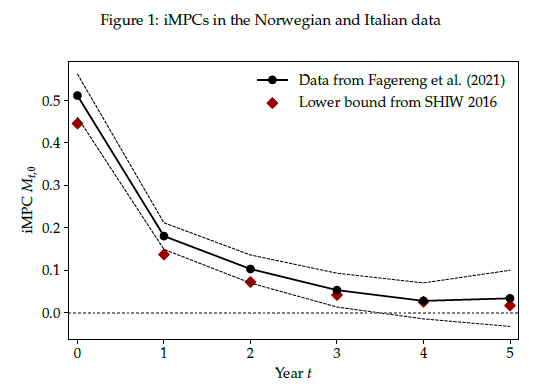
\includegraphics[width=0.65\textwidth]{data_evidence.png}
        \caption{Source: Auclert et al. (2024)}
    \end{figure}
\end{frame}


\begin{frame}{iMPCS visually}
    \begin{figure}
    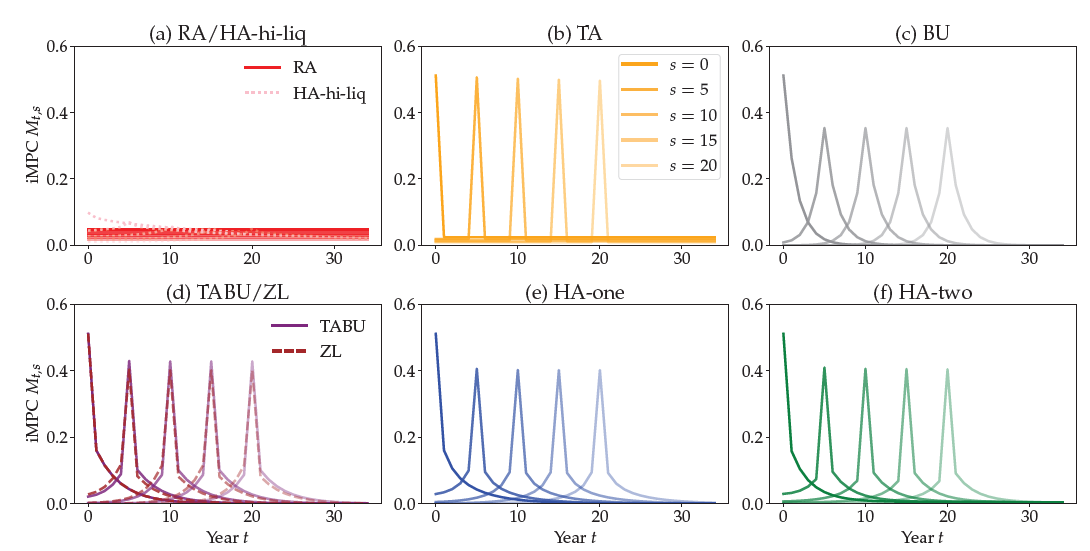
\includegraphics[width=1\textwidth]{impcs.png}
    \caption{Source: Auclert et al. (2024)}
    \end{figure}
        \end{frame}
    
    
    \begin{frame}{iMPCS visually}
        \begin{figure}
    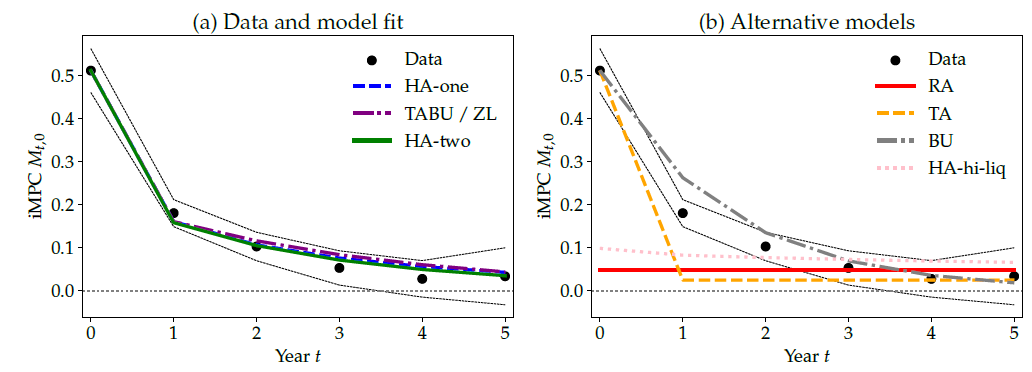
\includegraphics[width=1\textwidth]{impcs_data.png}
    \caption{Source: Auclert et al. (2024)}
    \end{figure}
    \end{frame}
    
    
    \begin{frame}{Balanced budget}
        \begin{itemize}
           \item In a old-fashioned Keynesian model, for $dg = dT$ we have $dy = dg$.
           \item Same holds in the IKC with $d\bm{g} = d\bm{T}$: \begin{align*}
             d\bm{y} & = d\bm{g} + \mathbf{M} d\bm{y} - \mathbf{M}  d\bm{T} \\
             & = d\bm{g} + \mathbf{M} d\bm{y} - \mathbf{M}  d\bm{g} \\
             & = \bp{\mathbf{I}-\mathbf{M}} d\bm{g} + \mathbf{M} d\bm{y}  \\
             \implies  & d\bm{y} = d\bm{g}
           \end{align*}
             \item This is a general property of the IKC. Holds irrespective of the details of the model, as long as we can write it in this form. 
        \end{itemize}
        \end{frame}
         
    \begin{frame}{Multipliers}
        \begin{figure}
        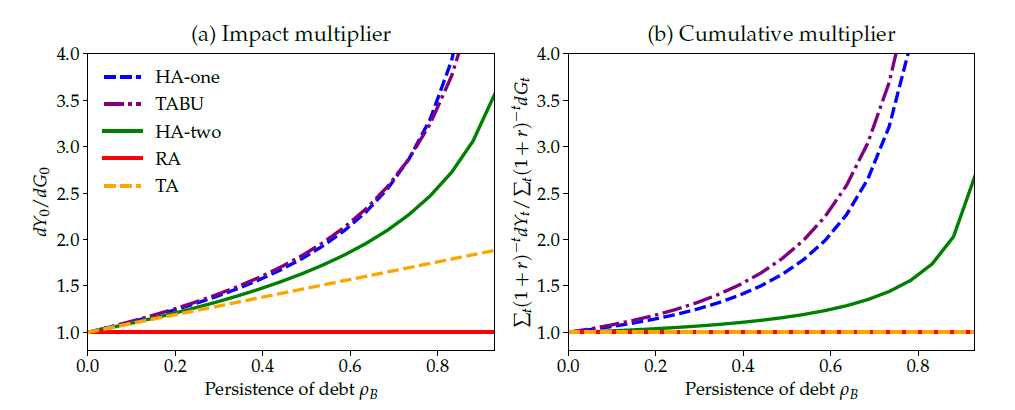
\includegraphics[width=1\textwidth]{multipliers.png}
        \caption{Source: Auclert et al. (2024)}
    \end{figure}
    \end{frame}

\begin{frame}
    \heading{Empirical results}
\end{frame}

\begin{frame}{Usual approaches}
    \begin{itemize}
    \item How to measure the multiplier? 
    \item Ramey (2019) distinguishes three main approaches: \begin{enumerate}
    \item aggregate country-level time series or panel estimates
    \item calibrated or estimated structural models 
    \item subnational geographic cross-section or panel estimates
    \end{enumerate}
    \item Common problem - identificiation: the time series approaches requires
    exogenous variation in policy. \begin{itemize} 
        \item  structural vector autoregressions and natural experiment methods,
    combined with narrative methods.
    \item instruments often have low correlation
    with the fiscal variable they are trying to explain
    \end{itemize}
\end{itemize}
\end{frame}

\begin{frame}{Usual approaches}
\begin{itemize}
\item The third approach estimates across subnational units (states or provinces).
\item These analyses have stronger identification due to more plausible assumptions and relevant instruments.
\item This approach does not directly lead to macroeconomic estimates.
\item Cross-sectional estimating equations include a constant term, netting out macroeconomic effects.
Parameters estimated are only relative effects: \emph{``If State A is awarded
\$1 more in defense prime contracts than the average state, by how much does its
employment change relative to the average state?''}
\item To infer national-level effects, researchers must use macroeconomic New Keynesian DSGE models.
\end{itemize}
\end{frame}

\begin{frame}{Usual approaches}
    \begin{itemize}
    \item What even is ``the'' multiplier?
    \item The effects of government spending on output are dynamic. Which ratio to use? 
    \item Blanchard and Perotti (2002) calculate the ratio of output response at horizon $h$ to the initial change of government spending. 
    \item Mountford and Uhlig (2009) calculate the ratio of the cumulative response of output to the cumulative response of government spending, discounted.
    \item Another issue: regressions are often in logs, need to convert it to levels. What is the right ratio?
\end{itemize}
    \end{frame}
    
    \begin{frame}[plain]{}
    
        \begin{figure}
        \begin{centering}
            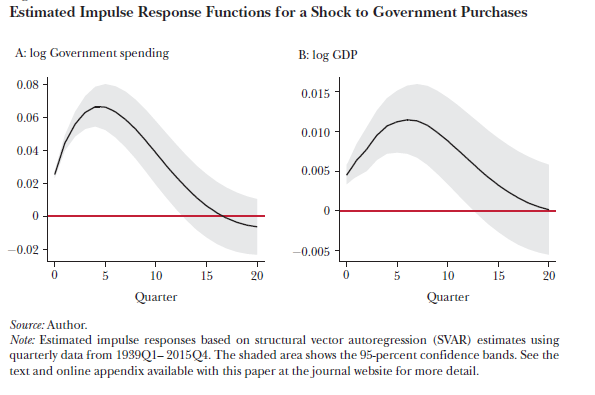
\includegraphics[width=0.8\textwidth]{ramey_2019_1.png}
        \par\end{centering}
        \caption{Ramey (2019)}
        
        \end{figure}
        \end{frame}

    \begin{frame}[plain]{}

        \begin{figure}
        \begin{centering}
            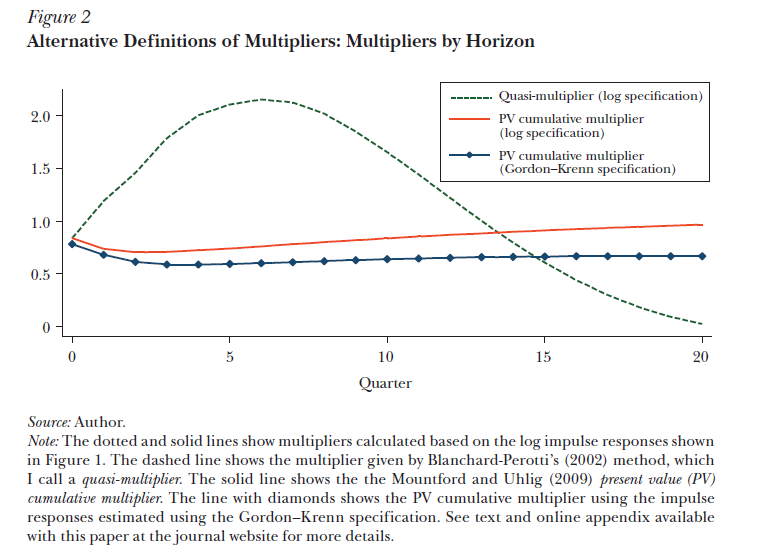
\includegraphics[width=0.8\textwidth]{ramey_2019_4.png}
        \par\end{centering}
        \caption{Ramey (2019)}
        
        \end{figure}
        \end{frame}

        %
        \begin{frame}{Shock identification}
        \begin{itemize}
        \item Narrative methods
        \begin{itemize}
        \item Military spending is often used. Defense spending is usually driven
        by political events and not macroeconomic events. Big increases in
        $g$ due to miliary buildups (eg. WW2). 
        \item Regress variables of interest on changes in miliary spending (Barro
        and Redlick 2009) or ``war dates''. 
        \item For example Ramey and Shapiro (1998) used narrative techniques to
        create a dummy variable capturing major military buildups. They read
        through Business Week in order to isolate the political events that
        led to the buildups in order to create a series that was exogenous
        to the current state of the economy.
        \item Potential problem with military events: other policies might be implemented
        at the same time, for example rationing or increases in taxes. 
        \item Timing of news vs spending?
        \end{itemize}
        \end{itemize}
        
        \end{frame}

    \begin{frame}[plain]{}
    
    \begin{figure}
    \begin{centering}
        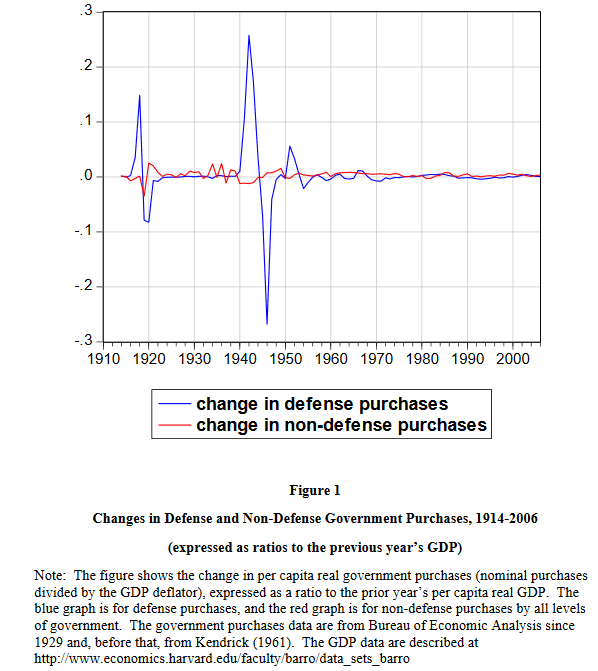
\includegraphics[width=0.5\textwidth]{barro_redlick.png}
    \par\end{centering}
    \caption{Barro, Redlick (2009)}
    \end{figure}
    \end{frame}

    %
    \begin{frame}{Shock identification}
    \begin{itemize}
    \item Structural Vector Autoregressions
    \begin{itemize}
    \item We will talk about in detail when we discuss monetary policy. Now
    just the basic idea.
    \item Run regression (VAR)
    \[
    Y_{t}=A_{1}Y_{t-1}+A_{2}Y_{t-2}+\cdots+U_{t}
    \]
    where $Y_{t}$ is a vector of variables at time $t$. For example:
    government purchases, taxes and GDP. 
    \item $U_{t}$ is a vector of residuals. We have to relate them to ``structural
    shocks''. To do so we impose restrictions. For example: unexpected
    changes in GDP do not lead to changes in purchases in the same quarter
    (it takes time to pass stimulus bill). 
    \item Then we track response of variables to ``structural shocks''
    \item Blanchard and Perotti (2002): gov. purchases not explained by some lagged variables $\rightarrow$ shocks.
    \item This can make use of ``narrative approach'' - just add ``war dummies''!
    \end{itemize}
    \end{itemize}
    \end{frame}
    %
    \begin{frame}[plain]{}
    \begin{figure}
    \begin{raggedright}
        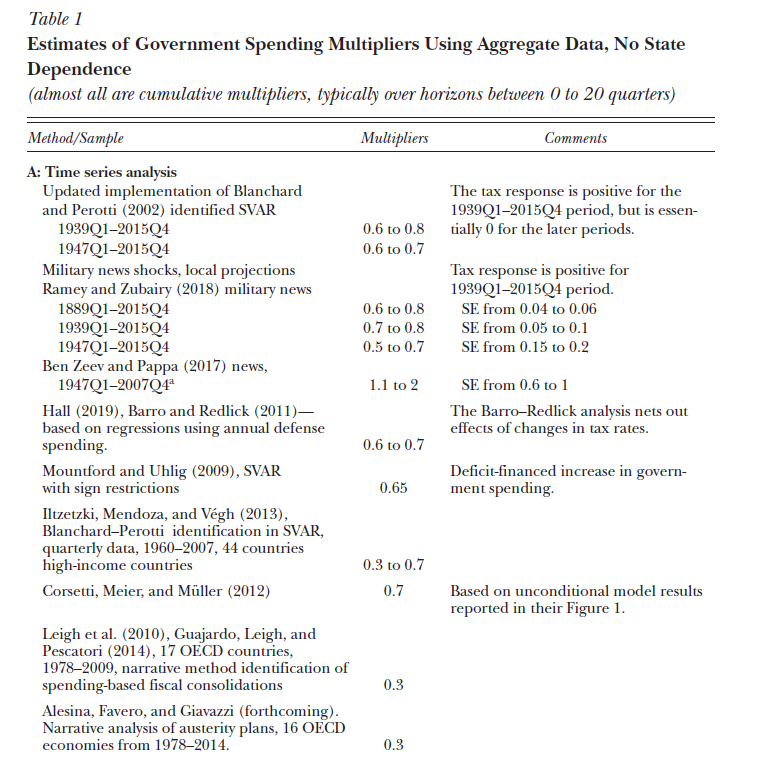
\includegraphics[width=0.55\textwidth]{ramey_2019_2.png}
    \par\end{raggedright}
    \caption{Ramey (2019)}
    
    \end{figure}
    
    \end{frame}

\begin{frame}[plain]{}
    \begin{figure}
    \begin{raggedright}
        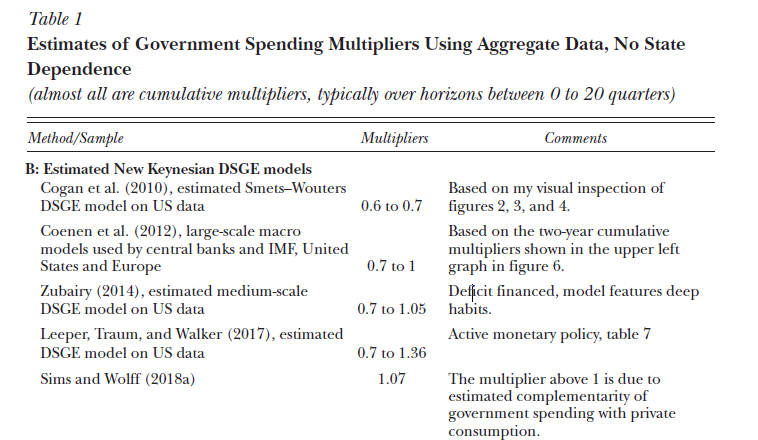
\includegraphics[width=0.55\textwidth]{ramey_2019_3.png}
    \par\end{raggedright}
    \caption{Ramey (2019)}
    
    \end{figure}
    
    \end{frame}

    \begin{frame}[plain]{}
        \begin{figure}
        \begin{raggedright}
            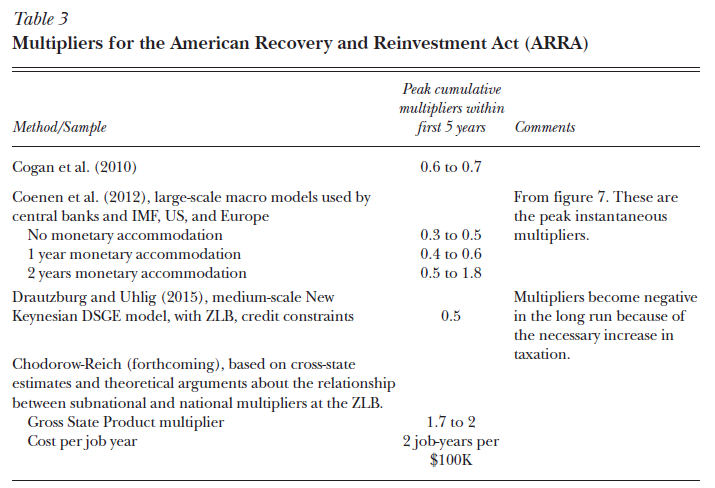
\includegraphics[width=0.55\textwidth]{ramey_2019_5.png}
        \par\end{raggedright}
        \caption{Ramey (2019)}
        
        \end{figure}
        
        \end{frame}
    
    \end{frame}

    \begin{frame}[plain]{}
        \begin{figure}
        \begin{raggedright}
            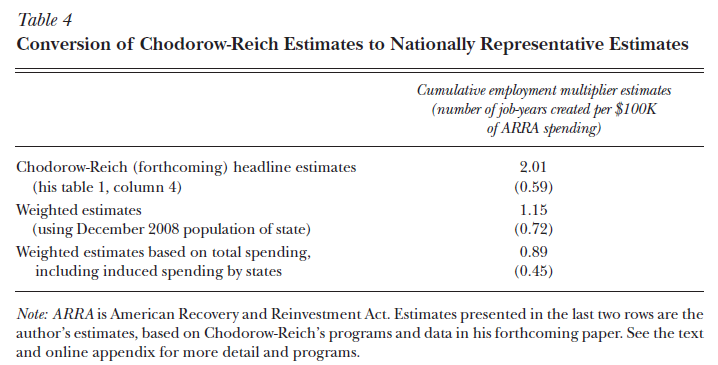
\includegraphics[width=0.55\textwidth]{ramey_2019_6.png}
        \par\end{raggedright}
        \caption{Ramey (2019)}
        
        \end{figure}
        
        \end{frame}
\end{document}